\documentclass[10pt,a4paper]{article}
\usepackage[margin=22mm]{geometry}
\usepackage[T1]{fontenc}
\usepackage{lmodern,amsmath,amssymb,booktabs,graphicx,tikz,hyperref,fvextra}
\usetikzlibrary{arrows.meta,positioning,calc,decorations.pathmorphing}
\definecolor{ink}{RGB}{20,53,78}
\hypersetup{colorlinks=true,urlcolor=ink,linkcolor=ink}
\setlength{\parindent}{0pt}
\setlength{\parskip}{5pt}
\emergencystretch=3em

\title{\color{ink}Two thermal zones with one temperature measurement}
\author{}
\date{Original learning collection -- November 2026}
\begin{document}
\begin{center}{\LARGE\color{ink}Two thermal zones with one temperature measurement}\\[5pt]{\small Original learning collection -- November 2026}\end{center}

\textbf{Evidence note.} Original teaching scenario. Numerical parameters are deliberately chosen for learning. All generated data and curves are synthetic; no physical measurement is asserted.
\section{Design brief}
Two hypothetical thermal zones obey $\dot x=Ax+Bu$ and $y=Cx$, with
\[
A=\begin{bmatrix}-0.15&0.05\\0.05&-0.10\end{bmatrix}\,\mathrm{s^{-1}},
\quad B=\begin{bmatrix}0.1\\0\end{bmatrix}\,\mathrm{K/(s\,W)},
\quad C=\begin{bmatrix}0&1\end{bmatrix}.
\]
Check controllability and observability. Choose feedback poles $-0.20,-0.35$, observer poles $-0.8,-1.0$ and a constant reference prefilter. Starting at $x(0)=[0.6,-0.4]^{\mathsf T}\,\mathrm{K}$ with zero estimate, regulate zone 2 to a $1\,\mathrm{K}$ rise.
\section{Physical system}
\begin{center}\resizebox{\ifdim\width>.98\linewidth.98\linewidth\else\width\fi}{!}{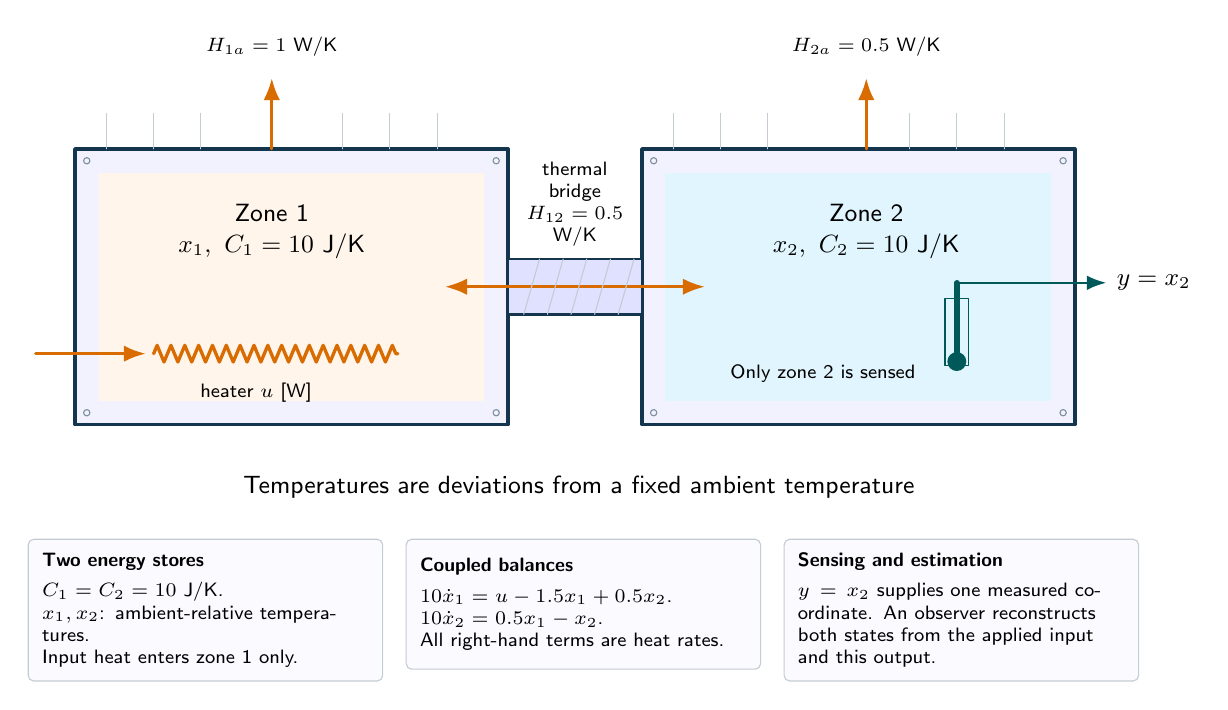
\begin{tikzpicture}[
font=\sffamily\small,>=Latex,line cap=round,line join=round,
wall/.style={draw=ink,line width=1.2pt,fill=blue!5},
water/.style={fill=cyan!25,draw=none},
metal/.style={draw=ink,fill=blue!12,line width=.9pt},
flow/.style={->,draw=blue!65!black,line width=1.2pt},
heat/.style={->,draw=orange!85!black,line width=1.1pt},
measure/.style={->,draw=teal!70!black,line width=.9pt},
dim/.style={<->,draw=ink!65,line width=.6pt},
spring/.style={draw=ink,decorate,decoration={coil,aspect=.5,segment length=4pt,amplitude=3pt}},
wire/.style={draw=ink,line width=1pt},
lab/.style={align=center,font=\sffamily\small},
smalllab/.style={align=center,font=\sffamily\scriptsize}]

\draw[wall](.6,.7)rectangle(6.1,4.2);
\draw[wall](7.8,.7)rectangle(13.3,4.2);
\fill[orange!8](.9,1)rectangle(5.8,3.9);
\fill[cyan!12](8.1,1)rectangle(13,3.9);
\draw[metal](6.1,2.1)rectangle(7.8,2.8);
\draw[heat,<->](5.3,2.45)--(8.6,2.45);
\node[smalllab]at(6.95,3.5){thermal\\bridge\\$H_{12}=0.5$\\W/K};
\draw[orange!85!black,line width=1.2pt,decorate,decoration={zigzag,segment length=5pt,amplitude=3pt}](1.6,1.6)--(4.7,1.6);
\draw[heat](.1,1.6)--(1.5,1.6);
\node[smalllab]at(2.9,1.1){heater $u$ [W]};
\node[lab]at(3.1,3.15){Zone 1\\$x_1,\ C_1=10$ J/K};
\node[lab]at(10.65,3.15){Zone 2\\$x_2,\ C_2=10$ J/K};
\draw[teal!70!black,line width=2pt](11.8,1.5)--(11.8,2.5);
\fill[teal!70!black](11.8,1.5)circle(.12);
\draw[measure](11.8,2.5)--(13.7,2.5)node[right]{$y=x_2$};
\draw[heat](3.1,4.2)--(3.1,5.1);
\draw[heat](10.65,4.2)--(10.65,5.1);
\node[smalllab]at(3.1,5.5){$H_{1a}=1$ W/K};
\node[smalllab]at(10.65,5.5){$H_{2a}=0.5$ W/K};
\node[lab]at(7,-.1){Temperatures are deviations from a fixed ambient temperature};
% REFINED EQUIPMENT DETAILS

% Distinct thermal masses and finite conductive contact.
\foreach \x in {1,1.6,2.2,4,4.6,5.2}{\draw[ink!25](\x,4.2)--(\x,4.65);}
\foreach \x in {8.2,8.8,9.4,11.2,11.8,12.4}{\draw[ink!25](\x,4.2)--(\x,4.65);}
\foreach \x in {6.3,6.6,6.9,7.2,7.5}{\draw[ink!25](\x,2.1)--(\x+.2,2.8);}
\foreach \x/\y in {.75/.85,.75/4.05,5.95/.85,5.95/4.05,7.95/.85,7.95/4.05,13.15/.85,13.15/4.05}{\draw[ink!55](\x,\y)circle(.04);}
\draw[teal!70!black](11.65,1.45)rectangle(11.95,2.3);
\node[smalllab]at(10.1,1.35){Only zone 2 is sensed};

\node[draw=ink!25,fill=blue!2,rounded corners=2pt,anchor=north west,text width=4.15cm,minimum height=1.65cm,inner sep=5pt,align=left,font=\sffamily\scriptsize]at(0.0,-0.75){\textbf{Two energy stores}\\[3pt]$C_1=C_2=10$ J/K.\\$x_1,x_2$: ambient-relative temperatures.\\Input heat enters zone 1 only.};
\node[draw=ink!25,fill=blue!2,rounded corners=2pt,anchor=north west,text width=4.15cm,minimum height=1.65cm,inner sep=5pt,align=left,font=\sffamily\scriptsize]at(4.8,-0.75){\textbf{Coupled balances}\\[3pt]$10\dot x_1=u-1.5x_1+0.5x_2$.\\$10\dot x_2=0.5x_1-x_2$.\\All right-hand terms are heat rates.};
\node[draw=ink!25,fill=blue!2,rounded corners=2pt,anchor=north west,text width=4.15cm,minimum height=1.65cm,inner sep=5pt,align=left,font=\sffamily\scriptsize]at(9.6,-0.75){\textbf{Sensing and estimation}\\[3pt]$y=x_2$ supplies one measured coordinate. An observer reconstructs both states from the applied input and this output.};
\end{tikzpicture}
}\par{\small Two thermal inventories are connected by a conductive bridge. Heating acts in the first zone and sensing in the second. These stated capacities and conductances reproduce the two-state model exactly under the lumped assumptions.}\end{center}
\section{What can be controlled and observed?}
The controllability matrix $[B\ AB]$ has determinant $0.0005$, while the observability matrix $[C;CA]$ for $C=[0\ 1]$ has determinant $-0.05$. Both are nonsingular. Heat injected into zone 1 can influence zone 2 through coupling, and the measured zone-2 temperature reveals the other state dynamically.
\section{Feedback and prefilter}
Choose $u=-K\hat x+Nr$. Pole placement yields $K$ such that $A-BK$ has eigenvalues $-0.20,-0.35$. For constant references,
\[N=-\left[C(A-BK)^{-1}B\right]^{-1}.\]
This formula gives unit DC reference gain only for the nominal model and no constant disturbance. It is not integral regulation.
\section{Observer and separation}
Use $\dot{\hat x}=A\hat x+Bu+L(y-C\hat x)$ and select $L$ by placing the eigenvalues of $A-LC$ at $-0.8,-1.0$. With error $e=x-\hat x$,
\[\begin{bmatrix}\dot x\\\dot e\end{bmatrix}=
\begin{bmatrix}A-BK&BK\\0&A-LC\end{bmatrix}\begin{bmatrix}x\\e\end{bmatrix}+
\begin{bmatrix}BN\\0\end{bmatrix}r.\]
The block triangular matrix shows why controller and observer eigenvalues combine without changing each other in the nominal linear model.
\section{Interpretation and limits}
Observer convergence can be faster than output regulation. Faster estimation is not free: sensor noise and unmodeled dynamics are amplified by aggressive observer gains. Heating/cooling limits and temperature-dependent heat transfer are omitted; negative incremental heat can require an active cooler or reduction from a positive bias.
\section{What to learn from the experiment}
State estimation and reference prefiltering solve different problems. A nominal prefilter does not replace integral action against unknown constant disturbances.
\section{System sketch}
\begin{center}\resizebox{\ifdim\width>.98\linewidth.98\linewidth\else\width\fi}{!}{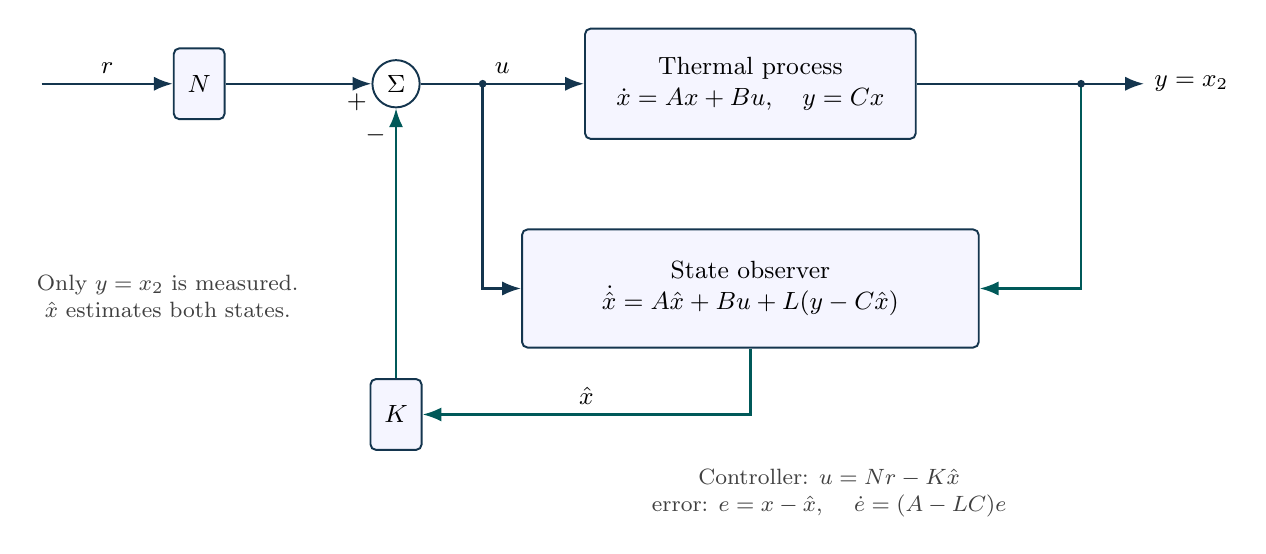
\begin{tikzpicture}[x=1cm,y=1cm,>=Latex,font=\small,
block/.style={draw=ink,fill=blue!4,rounded corners=2pt,minimum height=9mm,align=center,line width=.7pt,inner sep=5pt},
sum/.style={circle,draw=ink,fill=white,minimum size=6mm,inner sep=0pt,line width=.7pt},
sig/.style={->,draw=ink,line width=.85pt},
fb/.style={->,draw=teal!70!black,line width=.85pt},
dist/.style={->,draw=orange!75!black,line width=.85pt},
tap/.style={circle,fill=ink,inner sep=1.4pt},
note/.style={font=\footnotesize,align=center,text=black!75}]

\node[block](n)at(2,1.1){$N$};
\node[sum](u)at(4.5,1.1){$\Sigma$};
\node[block,minimum width=42mm,minimum height=14mm](p)at(9,1.1){Thermal process\\$\dot x=Ax+Bu,\quad y=Cx$};
\draw[sig](0,1.1)--node[above]{$r$}(n);
\draw[sig](n)--node[pos=.9,below]{$+$}(u);
\draw[sig](u)--node[above]{$u$}(p);
\draw[sig](p)--(14,1.1)node[right]{$y=x_2$};
\node[block,minimum width=58mm,minimum height=15mm](o)at(9,-1.5){State observer\\$\dot{\hat x}=A\hat x+Bu+L(y-C\hat x)$};
\draw[sig](5.6,1.1)--(5.6,-1.5)--(o.west);
\fill[ink](5.6,1.1)circle(1.4pt);
\draw[fb](13.2,1.1)--(13.2,-1.5)--(o.east);
\fill[ink](13.2,1.1)circle(1.4pt);
\node[block](k)at(4.5,-3.1){$K$};
\draw[fb](o.south)--(9,-3.1)--node[above]{$\hat x$}(k);
\draw[fb](k.north)--node[pos=.9,left]{$-$}(u.south);
\node[note]at(1.6,-1.6){Only $y=x_2$ is measured.\\$\hat x$ estimates both states.};
\node[note]at(10,-4.1){Controller: $u=Nr-K\hat x$\\error: $e=x-\hat x$, $\quad\dot e=(A-LC)e$};

\end{tikzpicture}
}
\par\small\refstepcounter{figure}\label{fig:system}\textbf{Figure \thefigure.} The observer receives both the applied control and measured output. Its estimated vector supplies state feedback; the prefilter sets nominal reference gain.\end{center}
\section{Executed computational evidence}
\VerbatimInput[fontsize=\small,breaklines=true]{results.txt}
\begin{center}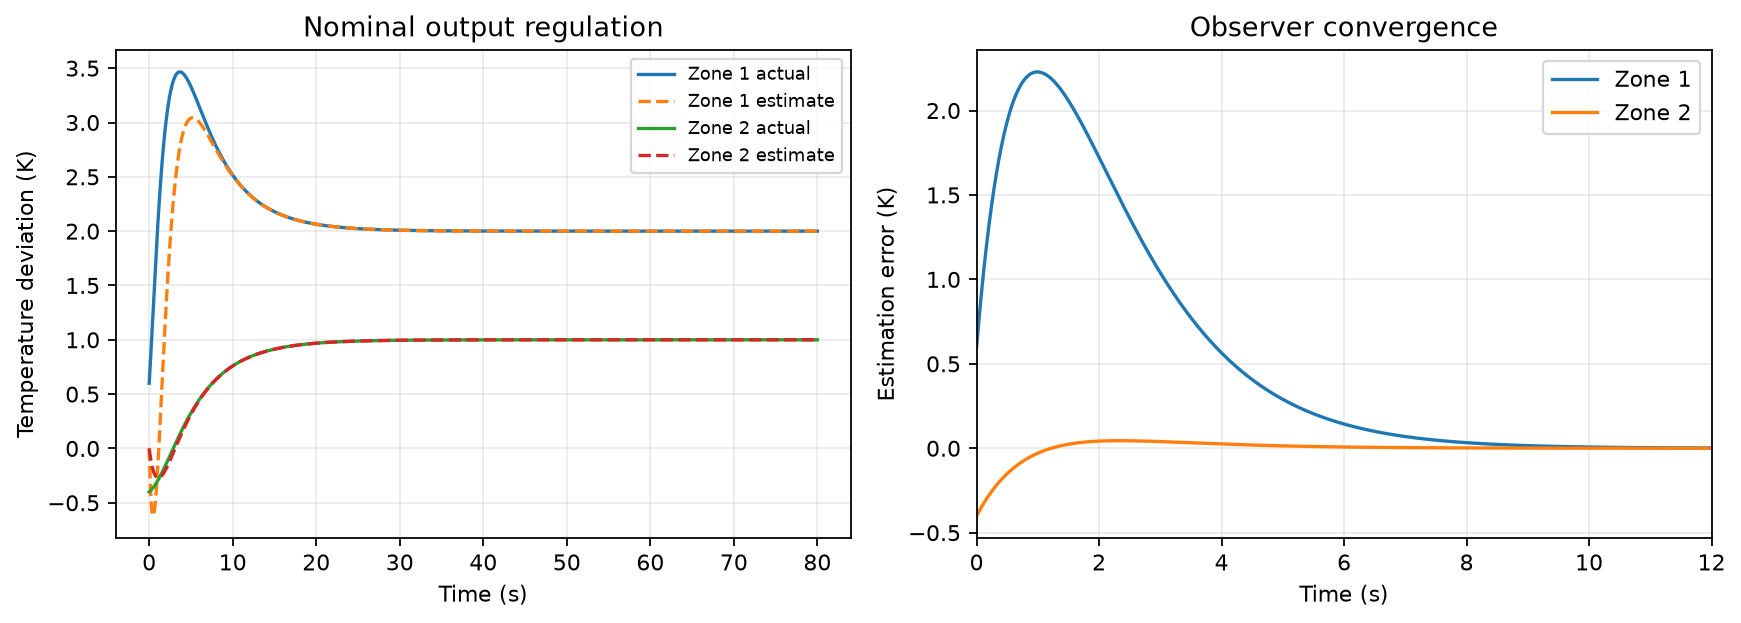
\includegraphics[width=\linewidth,height=.46\textheight,keepaspectratio]{response.png}\end{center}
\section{Method references}
The equations use standard balance laws and feedback-control methods. Further explanation: \url{https://apmonitor.com/pdc/} and \url{https://fbsbook.org/}. Implementation documentation: \url{https://python-control.readthedocs.io/en/0.10.2/}. See the repository reference catalog for individual topics and videos.
\end{document}
